\documentclass[11pt,a4paper]{article}
\usepackage[english]{babel}
\usepackage{amsmath} 
\usepackage{amssymb} 
\usepackage{mathtools} 
\usepackage{graphicx} 
\usepackage{fullpage}
\usepackage{color}
\usepackage[shortlabels]{enumitem}


\title{Statistical Learning Fall 2019\\ Homework 1\\}
\date{\vspace{-5ex}}



\begin{document}
\maketitle


\begin{description}
\item[Name Student:] Yizhen Dai
\item[Student Number:] S2395479
\end{description}


\section*{Introduction}

In this homework, we will apply linear regression on the housing data set, which concerns housing values in the suburbs of Boston. We will consider three ways of improving prediction accuracy: feature selection, ridge regression and the lasso. We will split the data set into two parts (training and test set), then fit the models on the training set (including choice of the best parameter using cross-validation) and test their performance on the separate test set.

\section*{Introductory analyses}

\begin{enumerate}[1.]
\item 	
The data set is downloaded from the website loaded to Jupyter Notebook. It is then divided into two parts, with the first 350 examples as a training set and the rest (156 examples) as a test set.

\item
After adding the dummy variable into training set as the intercept, we fit the least squares model to the training set.

\begin{figure}
  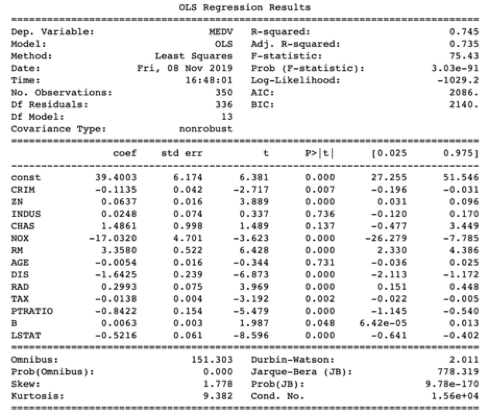
\includegraphics[width=\linewidth]{figure1.png}
  \caption{A boat.}
  \label{fig:boat1}
\end{figure}

Figure \ref{fig:boat1} shows a boat.

\end{enumerate}

\section*{Cross-validation and regularization}

Argue that the expressions on the left hand side of the equality evaluate to the real number, $\infty$ or $-\infty$ on the right hand side.



\noindent\textbf{\textbf{Solution:}}\\
\begin{enumerate}[a)]
	\item First, we consider the behaviour of the denominator. As $x$ approaches $-2$ from either the left or right side, $x + 2$ goes to $0$. The numerator $x^2 - 4$ also approaches $0$ as $x$ goes to $-2$. Rewriting the expression yields that for any $x \in \mathbb{R} \setminus \{2\}$,
	\begin{align*}
		\frac{x^2 - 4}{x+2} &= \frac{(x-2)(x+2)}{x+2} =x - 2,
	\end{align*}
	which tends to $-4$ as $x$ tends to $-2$ from either the left or the right side, which verifies what is asked of us.
	
	\item As $x$ approaches $-2$ from the left side, $x + 2$ approach $0$ from the left side (negative) and $\frac{1}{x + 2}$ approaches  $-\infty$.  As $x$ approaches $-2$ from the right side, $x + 2$ approach $0$ from the right side (positive) and $\frac{1}{x + 2} $ approaches  $\infty$. Therefore, 
	\begin{align*}
		\underset{x \searrow -2}{\lim} \frac{1}{x + 2} = +\infty,\\
		\underset{x \nearrow -2}{\lim} \frac{1}{x + 2} =- \infty
	\end{align*}
	which verifies the two-sided limit does not exist.
	
	\item The factor $x + 2$ approaches $2$ as x approaches $0$. Therefore, $ \frac{1}{x + 2}$ tends to $ \frac{1}{2}$  as x approaches $0$ from either the left or the right side, which verifies what is asked of us.
	
	\item Since $x \in (0, \infty)$, $\log_2 (x)$ only has right-hand limit at $x=0$. To meet $2^y = x$ , $y$ becomes larger and larger negative numbers as the values of $x$ approaches $0$ from the right. Give $x$ any natural number $c \in (0,1)$ , we get $\log_2 (c)$. There will always be another postive natural number $d < c$ gives a larger negative number $\log_2 (d)$. Therefore, we can say $\log_2 (x)$ has right-hand limit $-\infty$ at $x=0$.
\end{enumerate}


\section*{Model comparison}

\begin{enumerate}[(a)]

\item Comment on the magnitude of the differences.
\item Make an informed comparison against the least squares results, i.e. try to connect the theory to the results you have found.
\item Is any of the models useful to predict the outcome of housing prices? Explain why.
\item Compare the test-set error against the CV-error. Explain your findings.

best subset selection:
problems:
- computationally expensive
- not robust: high variance

ridge regression
- we need to standardize the features
- more stable/less variance than least squares for highly correlated features (ridge prefers equal weights)

Lasso
- find only most important features
- good for prediction and interpretation
- less variance than least squares




Consider the functions $f:\mathbb{R} \to \mathbb{R}$ defined by 
\begin{equation*}
f(x) = \begin{cases}
1 \text{ if } x \geq 2 \\
0 \text{ if } x < 2.
\end{cases}
\end{equation*}
and $g:\mathbb{R} \setminus \{ 2 \} \to \mathbb{R}$ defined by 
\begin{equation*}
g(x) = \frac{x^2 + 2x}{x^2 - 4} \text{ for } x \in \mathbb{R} \setminus \{ 2 \}.
\end{equation*}

Evaluate the specified (one or two sided) limits for the functions defined above. If their exist no limit, is the limit $-\infty$, $\infty$ or neither?


\begin{enumerate}[a)]
	\item \textbf{2 points:} Evaluate the (the right-side) limit $\underset{x \searrow 2}{\lim} f(x)$. Give an argument based on the informal definition of a limit.
	\item \textbf{2 points:} Evaluate the (the left-side) limit $\underset{x \nearrow 2}{\lim} f(x)$. Give an argument of why the based on the informal definition of a limit.
	\item \textbf{2 points:} Evaluate the limit $\underset{x \to 2}{\lim} f(x)$. \textbf{Hint:} Consider your answer to part (a) and (b).
	\item \textbf{2 points:}  $\underset{x \to 2}{\lim} g(x)$.
	\item \textbf{2 points:} $\underset{x \to \infty}{\lim} g(x)$.
\end{enumerate}

\noindent\textbf{\textbf{Solution:}}\\
\begin{enumerate}[a)]
	\item As $x$ approaches $2$ from the right side, $f(x)$ goes to $1$. Therefore  $\underset{x \searrow 2}{\lim} f(x) = 1$
	\item As $x$ approaches $2$ from the left side, $f(x)$ goes to $0$. Therefore  $\underset{x \nearrow 2}{\lim} f(x) = 0$
	\item Based on part (a) and (b), $f(x)$ goes to different values as $x$ approaches $2$ from either side. Since the one-sided limits are not equal even, the two-sided limit does not exist.
	\item Rewrite the expression for $f(x)$ as follows:
	\begin{equation*}
g(x) = \frac{x^2 + 2x}{x^2 - 4} 
= \frac{x*(x + 2)}{(x-2)*(x + 2)}
=\frac{x}{x-2}=\frac{1}{1-\frac{2}{x} }\text{ for } x \in \mathbb{R} \setminus \{-2, 2 \}.
	\end{equation*}
	The factor $1-\frac{2}{x}$ approaches $0$ as x approaches 2. Therefore, $g(x)$ has right-hand $\infty$ and left-hand $-\infty$ at $x=0$. We can put it as:	
	\begin{align*}
		\underset{x \searrow 2}{\lim} g(x) = +\infty,\\
		\underset{x \nearrow 2}{\lim} g(x)  =- \infty
	\end{align*}
	Since the one-sided limits are not equal even, the two-sided limit does not exist.

	\item As shown in part (d), $g(x) =\frac{1}{1-\frac{2}{x} }\text{ for } x \in \mathbb{R} \setminus \{-2, 2 \}$. The factor $1-\frac{2}{x}$ approaches $1$ as x approaches $\infty$. Therefore, $\underset{x \to \infty}{\lim} g(x)  = 1$.
\end{enumerate}

\section*{Exercise 4 (10 points)}

Consider the function $f:(0,\infty)\setminus \{ 4 \} \to \mathbb{R}$ defined by the equation
\begin{equation*}
 f(x) = \frac{\sqrt{x} - 2}{x^2 - 16} \text{ for } x \in (0,\infty) \setminus \{ 4 \}.
\end{equation*}
\begin{enumerate}[a)]
	\item \textbf{5 points:} Compute the limit $\underset{x \to 4}{\lim} f(x)$.
	\item \textbf{5 points:} Consider now for some number $L \in \mathbb{R}$ the function $g:\mathbb{R} \to \mathbb{R}$ defined by
	\begin{equation*}
	g(x) = \begin{cases}
	\frac{\sqrt{x} - 2}{x^2 - 16} \,\,\text{ for } x \in (0,\infty) \setminus \{ 4 \} \\
	L \,\,\text{ for } x= 4.
	\end{cases} 
	\end{equation*}
	For what value of $L$ is $g$ continuous on its entire domain?
\end{enumerate}


\noindent\textbf{\textbf{Solution:}}\\
\begin{enumerate}[a)]
	\item Rewriting the expression yields that for any $x \in (0,\infty) \setminus \{4\}$,
	\begin{align*}
		f(x)=\frac{\sqrt{x} - 2}{(x+4)(x-4)} = \frac{\sqrt{x} - 2}{(x+4)(\sqrt{x} + 2)(\sqrt{x} - 2)} =\frac{1}{(x+4)(\sqrt{x} + 2)} 
	\end{align*}
	which tends to $\frac{1}{32}$ as $x$ tends to $4$ from either the left or the right side. Therefore,
	\[\underset{x \to 4}{\lim} f(x) = \frac{1}{32}\]
	\item We say that a function $f$ is continuous at an interior point $c$ of its domain if  $\underset{x \to c}{\lim} f(x)= f(c) $. To make $g$ continous on its entire domain, $ \underset{x \to 4}{\lim} g(x) = g(4)$. Therefore, 
	\[ L = g(4)= \underset{x \to 4}{\lim} g(x) =\frac{1}{32} \]
\end{enumerate}

\section*{Exercise 5 (10 points)}
We call a function $f:\mathbb{R} \to \mathbb{R}$ a \textit{polynomial} if it satisfies
\begin{equation*}
f(x) = a_n x^n + a_{n-1} x^{n-1}+ \dots + a_1 x + a_0 \text{ for all } x \in \mathbb{R}
\end{equation*}
for some natural number $n$ and $a_n, a_{n-1}, \dots, a_0 \in \mathbb{R}$.

\vspace{12pt}

In this exercise we will show that any polynomial is a continuous function.

\begin{enumerate}[a)]
	\item \textbf{3 points:} Argue that the function $f:\mathbb{R} \to \mathbb{R}$ defined by $f(x) = x$ is continuous at every point of its domain. \textbf{Hint:} see the examples in 1.5 and recall the definition of a continuous function.
	\item \textbf{3 points:} Argue, using Theorem 2 of section 1.2 in the book, that $f:\mathbb{R} \to \mathbb{R}$ defined by $f(x) = x^2$ is continuous.  \textbf{Hint:} can we write $f$ as the product of two continuous functions?
	\item \textbf{2 points:} Argue in a similar way to part (b) that actually for any $n \in \mathbb{N}$ the function $f:\mathbb{R} \to \mathbb{R}$ defined by $f(x) = x^n$ is continuous.
	\item \textbf{2 points:} Now, using Theorem 2 twice more, conclude that any polynomial is a continuous function.
\end{enumerate}

\noindent\textbf{\textbf{Solution:}}\\
\begin{enumerate}[a)]
	\item For any number $c \in \mathbb{R}$, we want to show that there exists a $\delta > 0$ for each number $\epsilon >0 $ that for all $x \in \mathbb{N}\setminus \{c\}$ with $|x-c|<\delta$, it should hold that $|f(x)-f(c)|< \epsilon$. Set $  \delta=\epsilon \ $, $|f(x)-f(c)|=|x-c|<\delta = \epsilon$. It verifies $\underset{x \to c}{\lim} f(x)= f(c) $.  \\We say that a function $f$ is continuous at an interior point $c$ of its domain if  $\underset{x \to c}{\lim} f(x)= f(c) $. Therefore, $f(x) = x$ is continuous at every point of its domain.
	\item Define $g:\mathbb{R} \to \mathbb{R}$ by $g(x) = x$. Based on part 
(a), $g(x) = x$ is continuous at every point $c \in \mathbb{R}$ of its domain and $\underset{x \to c}{\lim} g(x)= c$. Since $f(x) = x^2 = g(x) * g(x)$, based on Theorem 2.3(Limit of a product), $\underset{x \to c}{\lim} f(x)= \underset{x \to c}{\lim} g(x) * \underset{x \to c}{\lim} g(x) = c^2$. It verifies $\underset{x \to c}{\lim} f(x)= f(c) $.  \\We say that a function $f$ is continuous at an interior point $c$ of its domain if  $\underset{x \to c}{\lim} f(x)= f(c) $.Therefore, $f(x) = x^2$ is continuous at every point of its domain.
	\item Define $g:\mathbb{R} \to \mathbb{R}$ by $g(x) = x$. Based on part 
(a), $g(x) = x$ is continuous at every point $c \in \mathbb{R}$ of its domain and $\underset{x \to c}{\lim} g(x)= c$. Since $f(x) = x^n = g(x)^n$, based on Theorem 2.6(Limit of a power), $\underset{x \to c}{\lim} f(x)= \underset{x \to c}{\lim} g(x) ^n= c^n$ for any number $c \in \mathbb{R}$. It verifies $\underset{x \to c}{\lim} f(x)= f(c) $. \\ We say that a function $f$ is continuous at an interior point $c$ of its domain if  $\underset{x \to c}{\lim} f(x)= f(c) $.Therefore, $f(x) = x^n$ is continuous at every point of its domain.
	\item Based on part(3), $f(x) = x^n$ is continuous at every point of its domain and $\underset{x \to c}{\lim} f(x)= c^n$. Set $g(x) = a  * x^n$, $a \in \mathbb{R}$. Based on Theorem 2.4(Limit of a multiple), $\underset{x \to c}{\lim} g(x)= a * c^n$ for any number $c \in \mathbb{R}$. It verifies $\underset{x \to c}{\lim} g(x)= g(c) $. \\ We say that a function $g$ is continuous at an interior point $c$ of its domain if  $\underset{x \to c}{\lim} g(x)= g(c) $.Therefore, $g(x) = a  * x^n$ is continuous at every point of its domain.\\
	
	For $f(x) = a_n x^n + a_{n-1} x^{n-1}+ \dots + a_1 x + a_0 \text{ for all } x \in \mathbb{R}$, based on Theorem 2.1(Limit of a sum), $\underset{x \to c}{\lim} f(x)= a_n c^n + a_{n-1} c^{n-1}+ \dots + a_1 c + a_0$ for any number $c \in \mathbb{R}$. It verifies $\underset{x \to c}{\lim} f(x)= f(c) $. \\ We say that a function $f$ is continuous at an interior point $c$ of its domain if  $\underset{x \to c}{\lim} f(x)= f(c) $. Therefore, $f(x) = a_n x^n + a_{n-1} x^{n-1}+ \dots + a_1 x + a_0 $ is continuous at every point of its domain.
\end{enumerate}

\section*{Bonus exercise (+5 points)}

\begin{enumerate}[a)]
	\item \textbf{+3 points:} Does the limit $\underset{x \to 0}{\lim} \sin (\frac{1}{x})$ exist? If not, is it $-\infty$, $\infty$ or neither? Base your reasoning on the behaviour of the function on the interval $(0,\delta)$, for $\delta >0$ a small (and shrinking) number.
	\item \textbf{+2 points:} Prove using the formal definition of a limit that $\underset{x \to 0}{\lim} [ x \cdot\sin (\frac{1}{x})]$ exists. \textbf{Hint:} Argue that $| x \cdot\sin (\frac{1}{x}) | \leq |x|$ based on the properties of the sine function. Then argue based on the formal definition as in Example 2 of section 1.5 in the book.
\end{enumerate}

\noindent\textbf{\textbf{Solution:}}\\
\begin{enumerate}[a)]
	\item To prove the limit $\underset{x \to 0}{\lim} \sin (\frac{1}{x})$ does not exist, we need to show no $L \in \mathbb{R}$ exists as $x$ goes to $0$ that for each number $\epsilon$ there exists a number $\delta$ such that for all $x \in \mathbb{R}$ with $|x - 0 | < \delta $ it holds that $|sin (\frac{1}{x}) - L | <  \epsilon $. \\
	\\As $x$ approaches $0$ from the right, $\frac{1}{x}$ approaches approaches $\infty$. Therefore,  $\sin (\frac{1}{x})$ will oscillate between $-1$ and $1$. Therefore. no $L$ can hold $|sin (\frac{1}{x}) - L | <  \epsilon $ for a small $\epsilon$.
	\item We want to show that as $x$ goes to $0$ that for each number $\epsilon$ there exists a number $\delta$ such that for all $x \in \mathbb{N} \setminus \{0\}$ with $|x - 0 | < \delta $ it holds that $|x \cdot sin (\frac{1}{x}) - 0 | <  \epsilon $. \\
	\\Since $ 0 \leq |sin (\frac{1}{x}) | \leq 1$, we can get $| x \cdot\sin (\frac{1}{x}) | = | x| \cdot |\sin (\frac{1}{x}) | \leq |x|$.\\
	\\Set $  \delta= \epsilon $, $|x \cdot sin (\frac{1}{x}) - 0 | <   |x| < \delta = \epsilon$. Hence it proves what is asked of us.


\end{enumerate}

\end{document}
